% !TEX root = ../finalReport.tex

\chapter{Methodology}
\label{chapter2}
\section{Core Engine Design: Representation and Computation}
\label{sec:core_engine_design}

Given Nonaga's branching factor of 440 (established in \cref{branching}), reaching a search depth of 3--4 within a human-playable time budget of a few seconds per move demands a game engine capable of evaluating tens of thousands of nodes per second. Every architectural decision in this chapter is evaluated against this core computational constraint.

\subsection{Board State Representation}
\label{subsec:board_state_representation}
A fundamental design choice in the development of the game engine was the internal representation of the Nonaga board. Traditional implementations of hexagonal board games often rely on 2D arrays or object-oriented graph structures. However, these approaches incur significant overhead and CPU cache-miss penalties during the millions of node evaluations required by deep adversarial search.

To achieve maximum computational throughput, a Bitboard architecture was implemented. By mapping the 19-cell hexagonal grid of Nonaga to an array of 64-bit integers, the entire game state is compressed. Consequently, complex operations such as move generation, tile movability status, and win-condition validation are reduced to highly efficient, CPU-native bitwise operations (AND, OR, XOR) that evaluate the board state in parallel against precomputed bitmasks. While the application of bitboards is well-documented for standard board geometries \cite{tannous2007avoiding} and has been explored for non-standard ones \cite{browne2014bitboards}, adapting this architecture to Nonaga's unique, dynamic topology represented a calculated engineering risk, as no prior work addressed a hexagonally-restructuring game board specifically. The primary risk was an increase in development time and architectural complexity, with the contingency that the geometric regularity of the hexagonal grid would permit a systematic derivation of the required bitmasks.

\section{Artificial Intelligence and Search Strategy}
\label{sec:ai_search_strategy}

\subsection{Adversarial Search Algorithm}
\label{subsec:adversarial_search}
While Monte Carlo Tree Search (MCTS) is a popular choice for games with high branching factors, an enhanced Minimax algorithm was selected for this project. Because Nonaga is heavily geometric, its strategic value is largely expressible through spatial features such as piece proximity and axial alignment, which are directly computable from the bitboard state, allowing a highly accurate heuristic evaluation function to be reliably constructed. Leveraging this domain knowledge via Minimax was estimated to provide a more deterministic and robust early-game performance than the randomized rollouts of standard MCTS, a conclusion supported by comparative studies in domains where reliable heuristics can be constructed \cite{SA2020survey, MCTSminimax}.

The primary decision-making agent utilizes this Minimax algorithm, significantly optimized via Alpha-Beta Pruning, Iterative Deepening, and a Transposition Table (TT) backed by Zobrist Hashing. Furthermore, the TT does more than just eliminate the redundant computation of identical board states; it serves as a highly efficient First-Move Ordering mechanism maximizing the efficiency of the Alpha-Beta pruning process. Instead of incurring the heavy computational overhead of dynamically sorting all possible legal moves at every node, the engine utilizes a Hash Move heuristic. By saving the hash of the best move encountered during the previous Iterative Deepening depth and retrieving it via the TT to evaluate first, the engine captures the vast majority of pruning benefits with a fraction of the algorithmic complexity.

\subsection{Evaluation Function}
\label{subsec:evaluation_function}
Because terminal win-states cannot be reached at shallow depths, the Minimax algorithm relies heavily on a parameterized heuristic evaluation function. This naturally integrates with Nonaga's highly geometric nature. Each parameter can be multiplied to a geometric feature of the board that can be efficiently derived from the bitboard. A linear evaluation function \cite{shannon1950programming} is particularly well-suited to this context, as it is computationally inexpensive to evaluate at every node of a deep search tree, whereas non-linear methods such as neural networks would impose a per-node latency incompatible with the depth required for competent play. Given Nonaga's significant branching factor, development resources were furthermore prioritised towards maximising search depth rather than evaluation complexity.

\section{Evaluation Function Optimization}

\subsection{GA Framework Design and Operator Selection}

To systematically optimize the weights of these parameters, a Genetic Algorithm (GA) framework was selected over traditional hill-climbing methodologies. The weights of the evaluation function are mutually dependent: the optimal value of one parameter is contingent on the values of the others. This interdependency creates a fitness landscape susceptible to premature convergence in gradient-following methods, making a population-based approach a more robust alternative \cite{goldberg1989genetic}.

A Random K-Opponent Tournament Scheduler was engineered, forcing genomes to compete against each other in self-play to determine their fitness. A unique challenge in optimizing heuristics for adversarial games is that fitness is entirely relative; a gene's performance is strictly dependent on the quality of its opponents. To mitigate this noise, the $K$ parameter (number of opponents) must be set as high as computationally acceptable to ensure a statistically significant fitness score. In practice, $K$ was determined empirically by incrementally increasing the number of opponents until the variance in fitness rankings across repeated runs stabilised. Roulette wheel selection and arithmetic crossover were selected as the GA operators, as these are well-established for continuous-valued parameter optimisation \cite{Katoch2021}; their concrete implementation is detailed in \cref{sec:ga_framework}.

It was recommended to benchmark the GA's convergence against an absolute "apex gene" found via brute-force search over a restricted domain (1--6 per parameter) \cite{assessor}. However, calculations revealed this to be unfeasible due to the estimated execution time and heavily neighborhood-dependent nature of the fitness landscape (further detailed in \cref{sec:hpc_feasibility}).

While advanced evolutionary strategies, specifically Linkage Learning, were proposed as a potential solution to this landscape dependency \cite{assessor}, their implementation was ultimately deemed out of scope. The core objective of the GA was to tune the evaluation function parameters to a highly performant standard, which the implemented baseline achieved successfully (as discussed in \cref{sec:ga_results}). For that reason, development resources were strategically reallocated to engine polishing and system optimization rather than over-engineering the evolutionary framework.

\section{System Architecture and Technology Stack}
\label{sec:system_architecture}

\subsection{Language Selection and Hybrid Integration}
\label{subsec:language_selection}
The overarching architectural goal was to deliver an interactive desktop client without compromising the extreme execution speeds required by the AI engine. Pure Python, while excellent for rapid UI prototyping via the PyGame library, was deemed fundamentally unsuitable for the core algorithmic engine. The Python Global Interpreter Lock (GIL) and the inherent overhead of dynamic object handling introduce severe bottlenecks when executing computationally dense bitwise operations and recursive tree searches \cite{beazley2010}.

To resolve this, a hybrid technology stack was engineered. The low-level Bitboard logic and Minimax core were strictly implemented in standard C, granting precise control over memory allocation and maximum instruction optimization. Python was retained exclusively for high-level orchestration, user interface rendering, and the GA tournament scheduling. Cython was utilized as the critical bridging layer, allowing the C-compiled backend to be exposed as native Python modules \cite{behnel2011cython}. This multi-language architecture cleanly separates the presentation layer from the algorithmic core, guaranteeing that both the interactive gameplay and the offline GA training pipelines execute against the exact same high-performance ruleset without rule drift or latency.

C was preferred over managed-runtime alternatives such as Java for the performance-critical kernel, as it avoids garbage collection pauses and provides the predictable, cache-friendly memory access critical for tight search loops \cite{wingqvist2022dod, arantes2025impact}. C++ was considered but rejected, as its additional abstraction overhead offered no measurable advantage over C for this narrowly scoped kernel. Existing proficiency with both Python and C further reduced development overhead and integration risk. The primary risk of this approach was the increase in development time and debugging complexity inherent to C, which lacks the high-level abstractions available in Python; this was mitigated by strictly limiting C code to the well-defined bitboard and search kernel, with Python retained for all higher-level logic.

The resulting component structure of the main game client, illustrating which classes invoke one another and the rationale for those dependencies, is shown in Figure~\ref{fig:classdiagram}.

\begin{figure}[H]
    \centering
    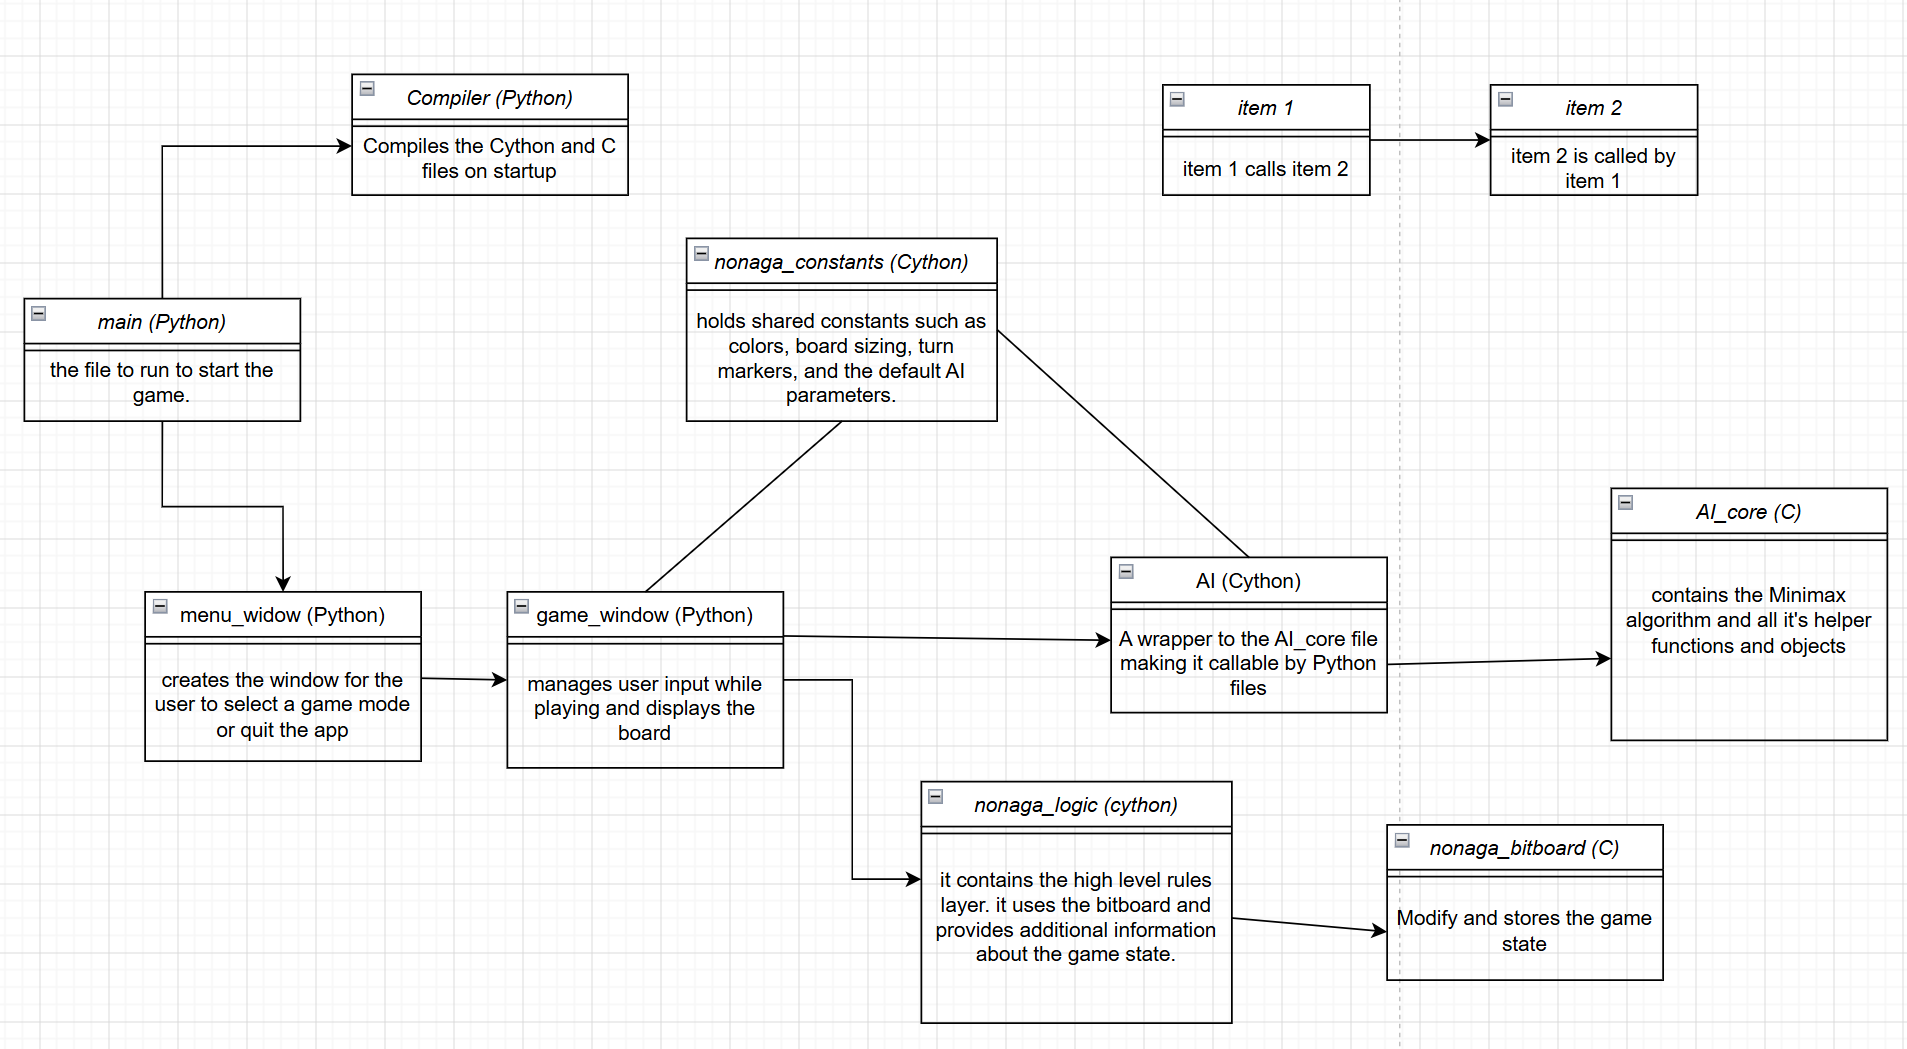
\includegraphics[width=0.85\textwidth]{pictures/Mthodology/class diagram.png}
    \caption{Class diagram of the main game client, illustrating the call dependencies between core software components.}
    \label{fig:classdiagram}
\end{figure}

\section{Project Management}

Throughout the project lifecycle, \texttt{git} was employed as the primary version control system to manage the evolving codebase, track granular changes, and maintain a secure repository. Development was structured around a feature-branch workflow, with each phase's deliverable developed and stabilised on a dedicated branch before integration into the main trunk. This ensured that regressions introduced during low-level optimisation (Phase 3) could be isolated without destabilising the working implementation from earlier phases.

Initially, a rigid, linear project plan was formulated in the Project Outline and Specification; however, early implementation phases revealed that this structure was overly abstracted and practically restrictive. The original plan operated on the flawed assumption of strict modular independence. In reality, the high degree of uncertainty in the exact implementation methods rendered the strict Waterfall approach implied in the plan nonviable.

Consequently, the project management strategy shifted to an adaptive, feature-driven Agile methodology. Development followed a verification-first discipline: each feature was considered complete only once it had been validated against a defined set of functional criteria, with custom diagnostic tooling developed specifically to support this process (detailed in \cref{sec:freemove}). The workflow followed a strict iterative loop: a target feature was engineered, rigorously verified against its functional requirements, and fully stabilized before continuous research dictated the selection and prioritization of the subsequent development target.

\subsection{Iterative Development Phases}

Because the project required continuous research and adaptation, the development lifecycle was structured around flexible objectives rather than strict time-boxed intervals. Each phase focused on delivering a functional, verifiable component of the overarching system. These phases map directly to the four project objectives outlined in \cref{sec:aim}: Phase 1 delivers the interactive GUI, Phases 2 and 3 deliver the high-performance engine and adversarial search, Phase 4 delivers the validation infrastructure, and Phase 5 delivers the GA optimisation pipeline.

\begin{itemize}
    \item \textbf{Phase 1: Core Mechanics and Visualization:} The initial focus was establishing a ground-truth representation of the game. The core rules of Nonaga were implemented in Python, paired with an interactive PyGame graphical user interface. By the end of this phase, human players could execute a valid game from start to finish, establishing a reliable baseline for future AI integration.

    \item \textbf{Phase 2: Adversarial Search Integration:} With a valid state representation in place, the focus shifted to algorithmic decision-making. By the end of this phase, the Minimax algorithm, enhanced with alpha-beta pruning, was successfully implemented to evaluate game trees.

    \item \textbf{Phase 3: Low-Level Optimization:} The objective of this phase was to minimize execution latency, thereby incrementally increasing the permissible search depth of the AI. By the end of this phase, the AI achieved a stable search depth of 3 within a pragmatic execution timeframe (a few seconds per move). This phase encompassed the language migration of performance-critical loops from pure Python to Cython/C, alongside the integration of bitboards, Transposition Tables, and move-ordering heuristics.

    \item \textbf{Phase 4: Diagnostic Tooling and Verification:} Custom diagnostic UI tools (detailed in \cref{sec:freemove}) were developed to manually verify the functional validity of the underlying engine modifications. This phase was introduced to establish a robust debugging infrastructure, facilitating the immediate isolation of logical regressions and minimizing subsequent debugging overhead as the architecture grew in complexity.

    \item \textbf{Phase 5: Evolutionary Tuning and Profiling:} The final phase focused on maximizing the AI's heuristic accuracy and computational efficiency. By the end of this phase, a modular Genetic Algorithm framework was constructed to automate the tuning of evaluation weights, resulting in a highly proficient artificial opponent.
\end{itemize}

This phase-driven approach provided the necessary flexibility to adapt to emergent technical challenges. Rather than adhering strictly to predetermined milestones, development iteratively cycled back to previous phases to address critical bottlenecks such as returning to core optimization (Phase 3) when subsequent heuristic tuning (Phase 5) revealed underlying performance constraints. Ultimately, the priority was to engineer a robust, high-performing AI, justifying deviations from the initial, rigid project specification.

\subsection{Scope Management}
As advised during the interim progress review, a pragmatic approach to scope management was adopted \cite{assessor}. Rather than expanding the project horizontally to encompass distributed cloud computing or widespread multi-platform deployment, development deliberately prioritized the deep optimization and polishing of the existing core architecture. This targeted focus ensured that the underlying AI engine and the local tuning frameworks achieved a rigorous standard of performance and stability without stretching the project's resources too thin.